\section{Pumps and Valves}
The addition of pumps, turbines, and valves increases some of the complexity for a network simulator.
Valves and other fittings like elbows and such, that have a fixed setting are modeled as links and the resulting equations look much like pipe loss equations.

Pumps while also logically categorized as links are more complex because their head loss behavior is firstly negative -- that is they add head to a flow system, and their ability to actually function is governed by their own performance curve.   First we will reviwe the modified Bernoulli equation again and then construct a prototype pump function to add to the program and simulate pump performance.

\subsection{Energy Loss (along a link)}
Equation \ref{eqn:closed-conduit-energy-equation} is the one-dimensional steady flow form of the energy equation typically applied for pressurized conduit hydraulics.
 
\begin{equation}
\frac{p_1}{\rho g}+\alpha_1 \frac{V_1^2}{2g} + z_1 + h_p =
\frac{p_2}{\rho g}+\alpha_2 \frac{V_2^2}{2g} + z_2 + h_t + h_l
\label{eqn:closed-conduit-energy-equation}
\end{equation}

where $\frac{p}{\rho g}$ is the pressure head at a location, $\alpha \frac{V^2}{2g}$ is the velocity head at a location, $z$ is the elevation, $h_p$ is the added head from a pump, $h_t$ is the added head extracted by a turbine, and $h_l$ is the head loss between sections 1 and 2.   Figure \ref{fig:closed-conduit-energy} is a sketch that illustrates the various components in Equation \ref{eqn:closed-conduit-energy-equation}.

\begin{figure}[h!] %  figure placement: here, top, bottom, or page
   \centering
   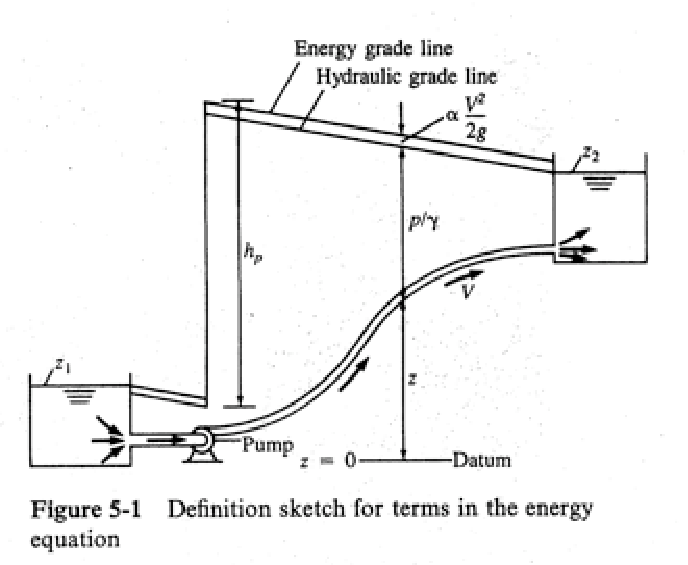
\includegraphics[width=4in]{./10-PumpsAndValves/closed-conduit-energy.pdf} 
   \caption{Definition sketch for energy equation}
   \label{fig:closed-conduit-energy}
\end{figure}

In network analysis this energy equation is applied to a link that joins two nodes.
Pumps and turbines would be treated as separate components (links) and their hydraulic behavior must be supplied using their respective pump/turbine curves.

\subsubsection{Added Head --- Pumps}
The head supplied by a pump is related to the mechanical power supplied to the flow.   Equation \ref{eqn:pump-power} is the relationship of mechanical power to added pump head.
\begin{equation}
\eta P=Q\rho g h_p
\label{eqn:pump-power}
\end{equation}
where the power supplied to the motor is $P$ and the  ``wire-to-water'' efficiency is $\eta$.

If the relationship is re-written in terms of added head\footnote{A negative head loss!} the pump curve is 
\begin{equation}
h_p = \frac{\eta P}{Q\rho g}
\label{eqn:pump-curve22}
\end{equation}

Figure \ref{fig:PumpCurve} is a typical pump curve depicting the kind of information available from a manufacturer of a pump.

\begin{figure}[h!] %  figure placement: here, top, bottom, or page
   \centering
   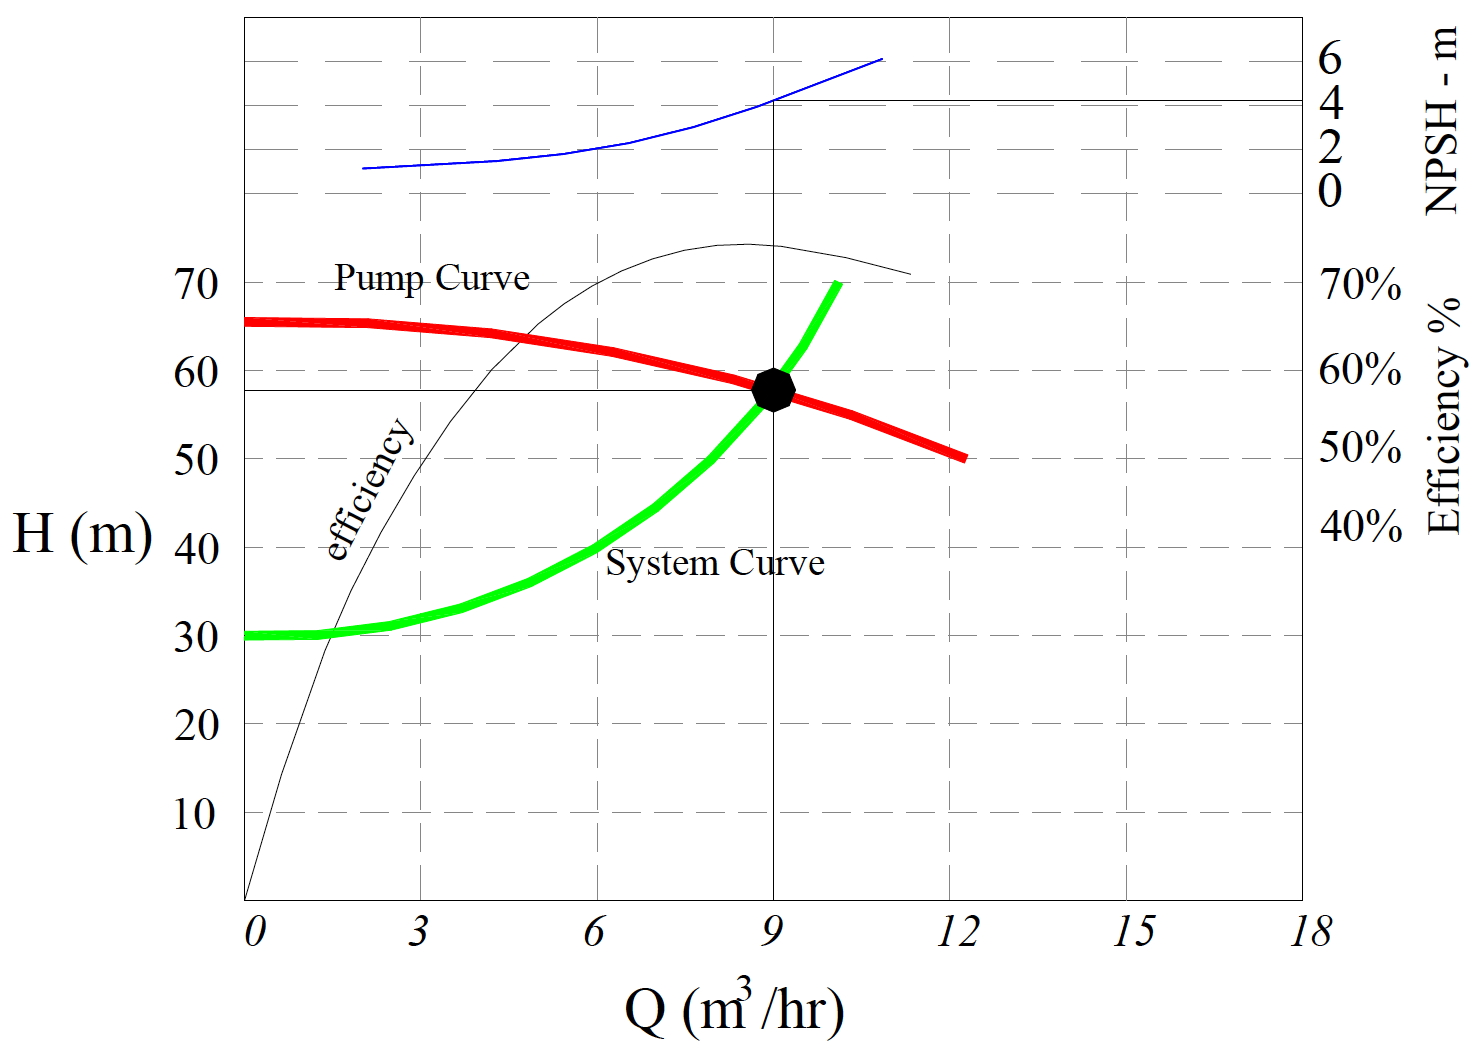
\includegraphics[width=4in]{./10-PumpsAndValves/PumpCurve.jpg} 
   \caption{Pump Curve}
   \label{fig:PumpCurve}
\end{figure}

In introductory fluid mechanics we spend effort to match the pump curve to the system curve (head losses in our distribution system) and that match tells us how the pump-system combination should function.   
The pump curve relationship, as well as Equation \ref{eqn:pump-curve22}, illustrates that as discharge increases (for a fixed power) the added head decreases.
Power scales at about the cube of discharge, so pump curves for computational application typically have a mathematical structure like
\begin{equation}
h_p =  H_{\text{shutoff}} - K_{\text{pump}}Q^{\text{exponent}}
\label{eqn:pump-curve-33}
\end{equation}
In computational hydraulics we will need to represent the added as a head loss term (with opposite sign), and the functional form represented by Equation \ref{eqn:pump-curve-33} is a good starting point.  
Practical (professional) programs will allow the curve to be represented in a tabular form and will use interpolation (just like our examples earlier) to specify the added head at a particular flow rate.

The next example will illustrate how to add pumps into the model.

\textbf{Example 1: Pipe network with pumps}\\
Figure \ref{fig:pipe-net-pumps} is a sketch of the problem that will be used.  
The network supply is the fixed-grade node in the upper left hand corner of the drawing -- in this example its head is set at zero.  
The remaining nodes (N1 -- N4) have demands specified as the purple outflow arrows.
The pipes are labeled (P2 -- P6), and the red arrows indicate a positive flow direction, that is, if the flow is in the indicated direction, the numerical value of flow (or velocity) in that link would be a positive number.
\begin{figure}[h!] %  figure placement: here, top, bottom, or page
   \centering
   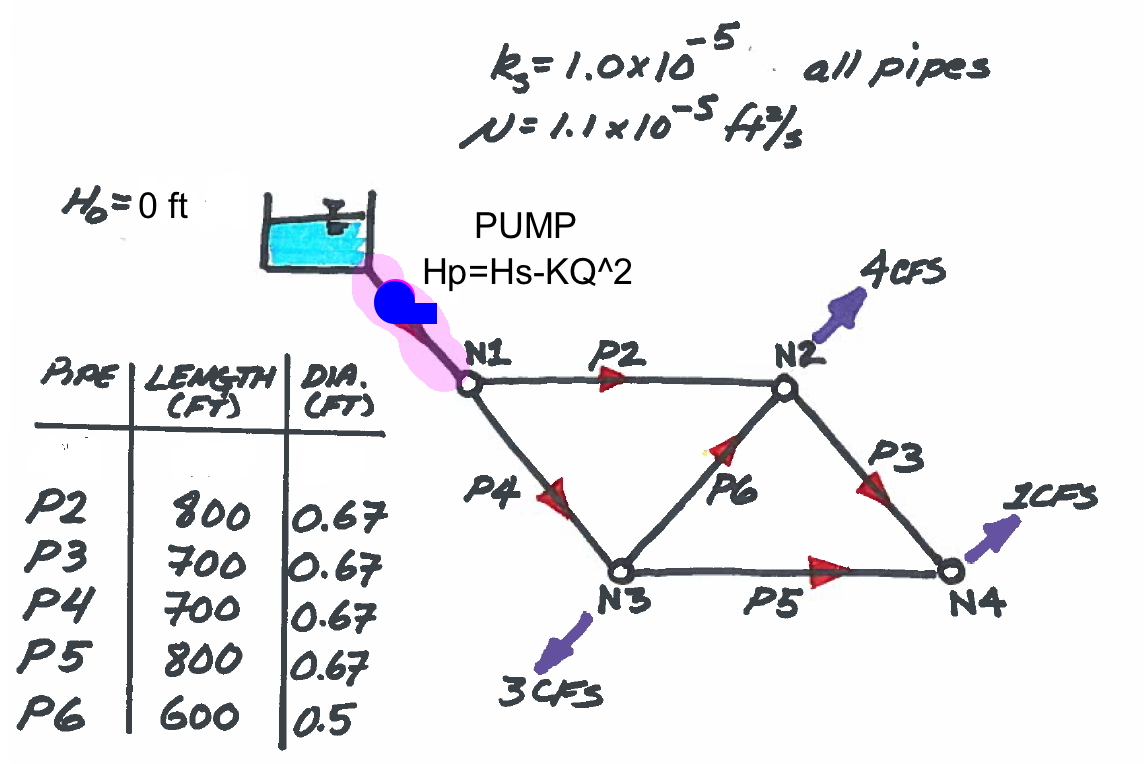
\includegraphics[width=4in]{./10-PumpsAndValves/pipe-net-pumps.jpg} 
   \caption{Pipe Network with a Pump}
   \label{fig:pipe-net-pumps}
\end{figure}
The pump replaces pipe (P1) from the previous version of this example.  
We will use the observation that we really only need to identify which links are pumps, substitute in the correct added head component and then solve the system as in the earlier example.   

We have to specify how the pump curve will be represented.
In this example we will use a functional form.
\begin{equation}
h_p(Q) = H_{shutoff} - K_{pump}\times Q^{n}
\end{equation}

For this example we will use the following numerical values for the pump function:
$H_{shutoff} = 104.54~\text{feet}$, $K_{pump} = 0.25~\text{feet}/cfs^2$, and $n = 2$.

The $h_p(Q)$ is actually written as an added head factor, just like the friction factor, so we will use absolute values of flow so the term at each computational step can be placed in the augmented maxrix as if it were a head loss term; the solver will not know the difference.

The actual functional form employed is
\begin{equation}
h_p(Q) = [H_{shutoff}/|Q| - K_{pump}\times |Q^{}|]Q
\end{equation}

As before the sign of $Q$ at the solution conveys flow direction.   
The program example does not trap the potential divide by zero error $H_{shutoff}/|Q|$, but one could test for zero flow, and just apply the shutoff head.  
Listing \ref{lst:PipelineWithPump} implements the prototype function described above.  

\begin{lstlisting}[caption=R Code to pump prototype function \\ , label=lst:PipelineWithPump]
.....
# Pump Curve factor function
p_factor <- function(shutoff,constant,exponent,flow){
  p_factor <- shutoff/abs(flow) - constant*abs(flow^(exponent-1))
  return(p_factor)
}
\end{lstlisting}   

Next we have to read in the pump characteristics, I decided to just have pumps replace links (so I won't have to rebuild a node-arc-incidence matrix), so the pump characteristics are 
\begin{enumerate}
\item Link ID -- the index of the pipe that is replaced by a pump.
\item Shutoff head.
\item $K_{pump}$.
\item Exponent on the pump curve, $n$.  Typically it will be larger than $1.0$.  
\end{enumerate}

Listing \ref{lst:PipelineWithPump2} implements the reads from the input file, and builds the pump matrix.  

\begin{lstlisting}[caption=R Code to include pumps in a pipeline network \\ , label=lst:PipelineWithPump2]
# Read Input Data Stream from File
zz <- file("PipeNetwork.txt", "r") # Open a connection named zz to file named PipeNetwork.txt
pumpCount <- as.numeric(readLines(zz, n = 1, ok = TRUE, warn = TRUE,encoding = "unknown", skipNul = FALSE))
nodeCount <- as.numeric(readLines(zz, n = 1, ok = TRUE, warn = TRUE,encoding = "unknown", skipNul = FALSE))
.....
rhs_true <- (readLines(zz, n = 1, ok = TRUE, warn = TRUE,encoding = "unknown", skipNul = FALSE))
pumps <- (readLines(zz, n = pumpCount, ok = TRUE, warn = TRUE,encoding = "unknown", skipNul = FALSE))
close(zz) # Close connection zz
.....
pumps <-as.numeric(unlist(strsplit(pumps,split=" ")))
# convert nodearcs a matrix
# We will need to augment this matrix for the actual solution -- so after augmentation will deallocate the memory
nodearcs <-matrix(nodearcs,nrow=nodeCount,ncol=pipeCount,byrow = TRUE)
pumps <-matrix(pumps,nrow=pumpCount,ncol=4,byrow=TRUE)
.....
\end{lstlisting}   

Next we will have to compute the added head factor at each step, just like the friction factor, and we will overwrite the pipe that the pump replaces.\footnote{This approach is decidedly a hack for illustration purposes.  A more advanced program would probably just treat everything as a link and use a similar database build structure to determine if a link is a head loss or head add link.  My reasoning is that there will be fewer pumps than pipes in any system, so overwriting a fictitious pipe is not too much trouble.}

Listing \ref{lst:PipelineWithPump3} implements the computation of the added head factor, and the pump selection factor.  

\begin{lstlisting}[caption=R Code to include pumps in a pipeline network \\ , label=lst:PipelineWithPump3]
.................
 # compute the current pump factor
 if(pumpCount > 0){
  for (i in 1:pumpCount)
    {
      addedhead[i] <- p_factor(pumps[i,2],pumps[i,3],pumps[i,4],flowguess[pumps[i,1]]) 
    }
  }
# build the function matrix
 # operate on the lower left partition of the matrix
 istart <- nodeCount+1
 iend <- nodeCount+pipeCount
 jstart <- 1
 jend <- flowCount
 for (i in istart:iend ){
   for(j in jstart:jend ){
     if ((i-istart+1) == j)  {augmentedMat[i,j] <- -1*lossfactor[j];
      if(pumpCount > 0){
        for(ipump in 1:pumpCount) {
          if(j == pumps[ipump,1]) augmentedMat[i,j] <- addedhead[ipump]
        }
      }
    }
   }
 }
# print(augmentedMat)
..................
\end{lstlisting}   

The remainder of the code is unchanged.
Listing \ref{lst:InputWithPump} illustrates the changes in the input file.
We have added a row to indicate how many pumps will be used as the first record in the file.
The last record after the right-hand side vector is the pump characteristics; one row for each pump.
The scripts also test if there are zero pumps and skip code as needed.
Observe we still preserve Link \#1 data because its part of the node-arc matrix, but the length and diameter of the link is irrelevant (but need to be non-zero because we compute friction factors as if there were a pipe, but never use them.

\begin{figure}[h!] %  figure placement: here, top, bottom, or page
   \centering
   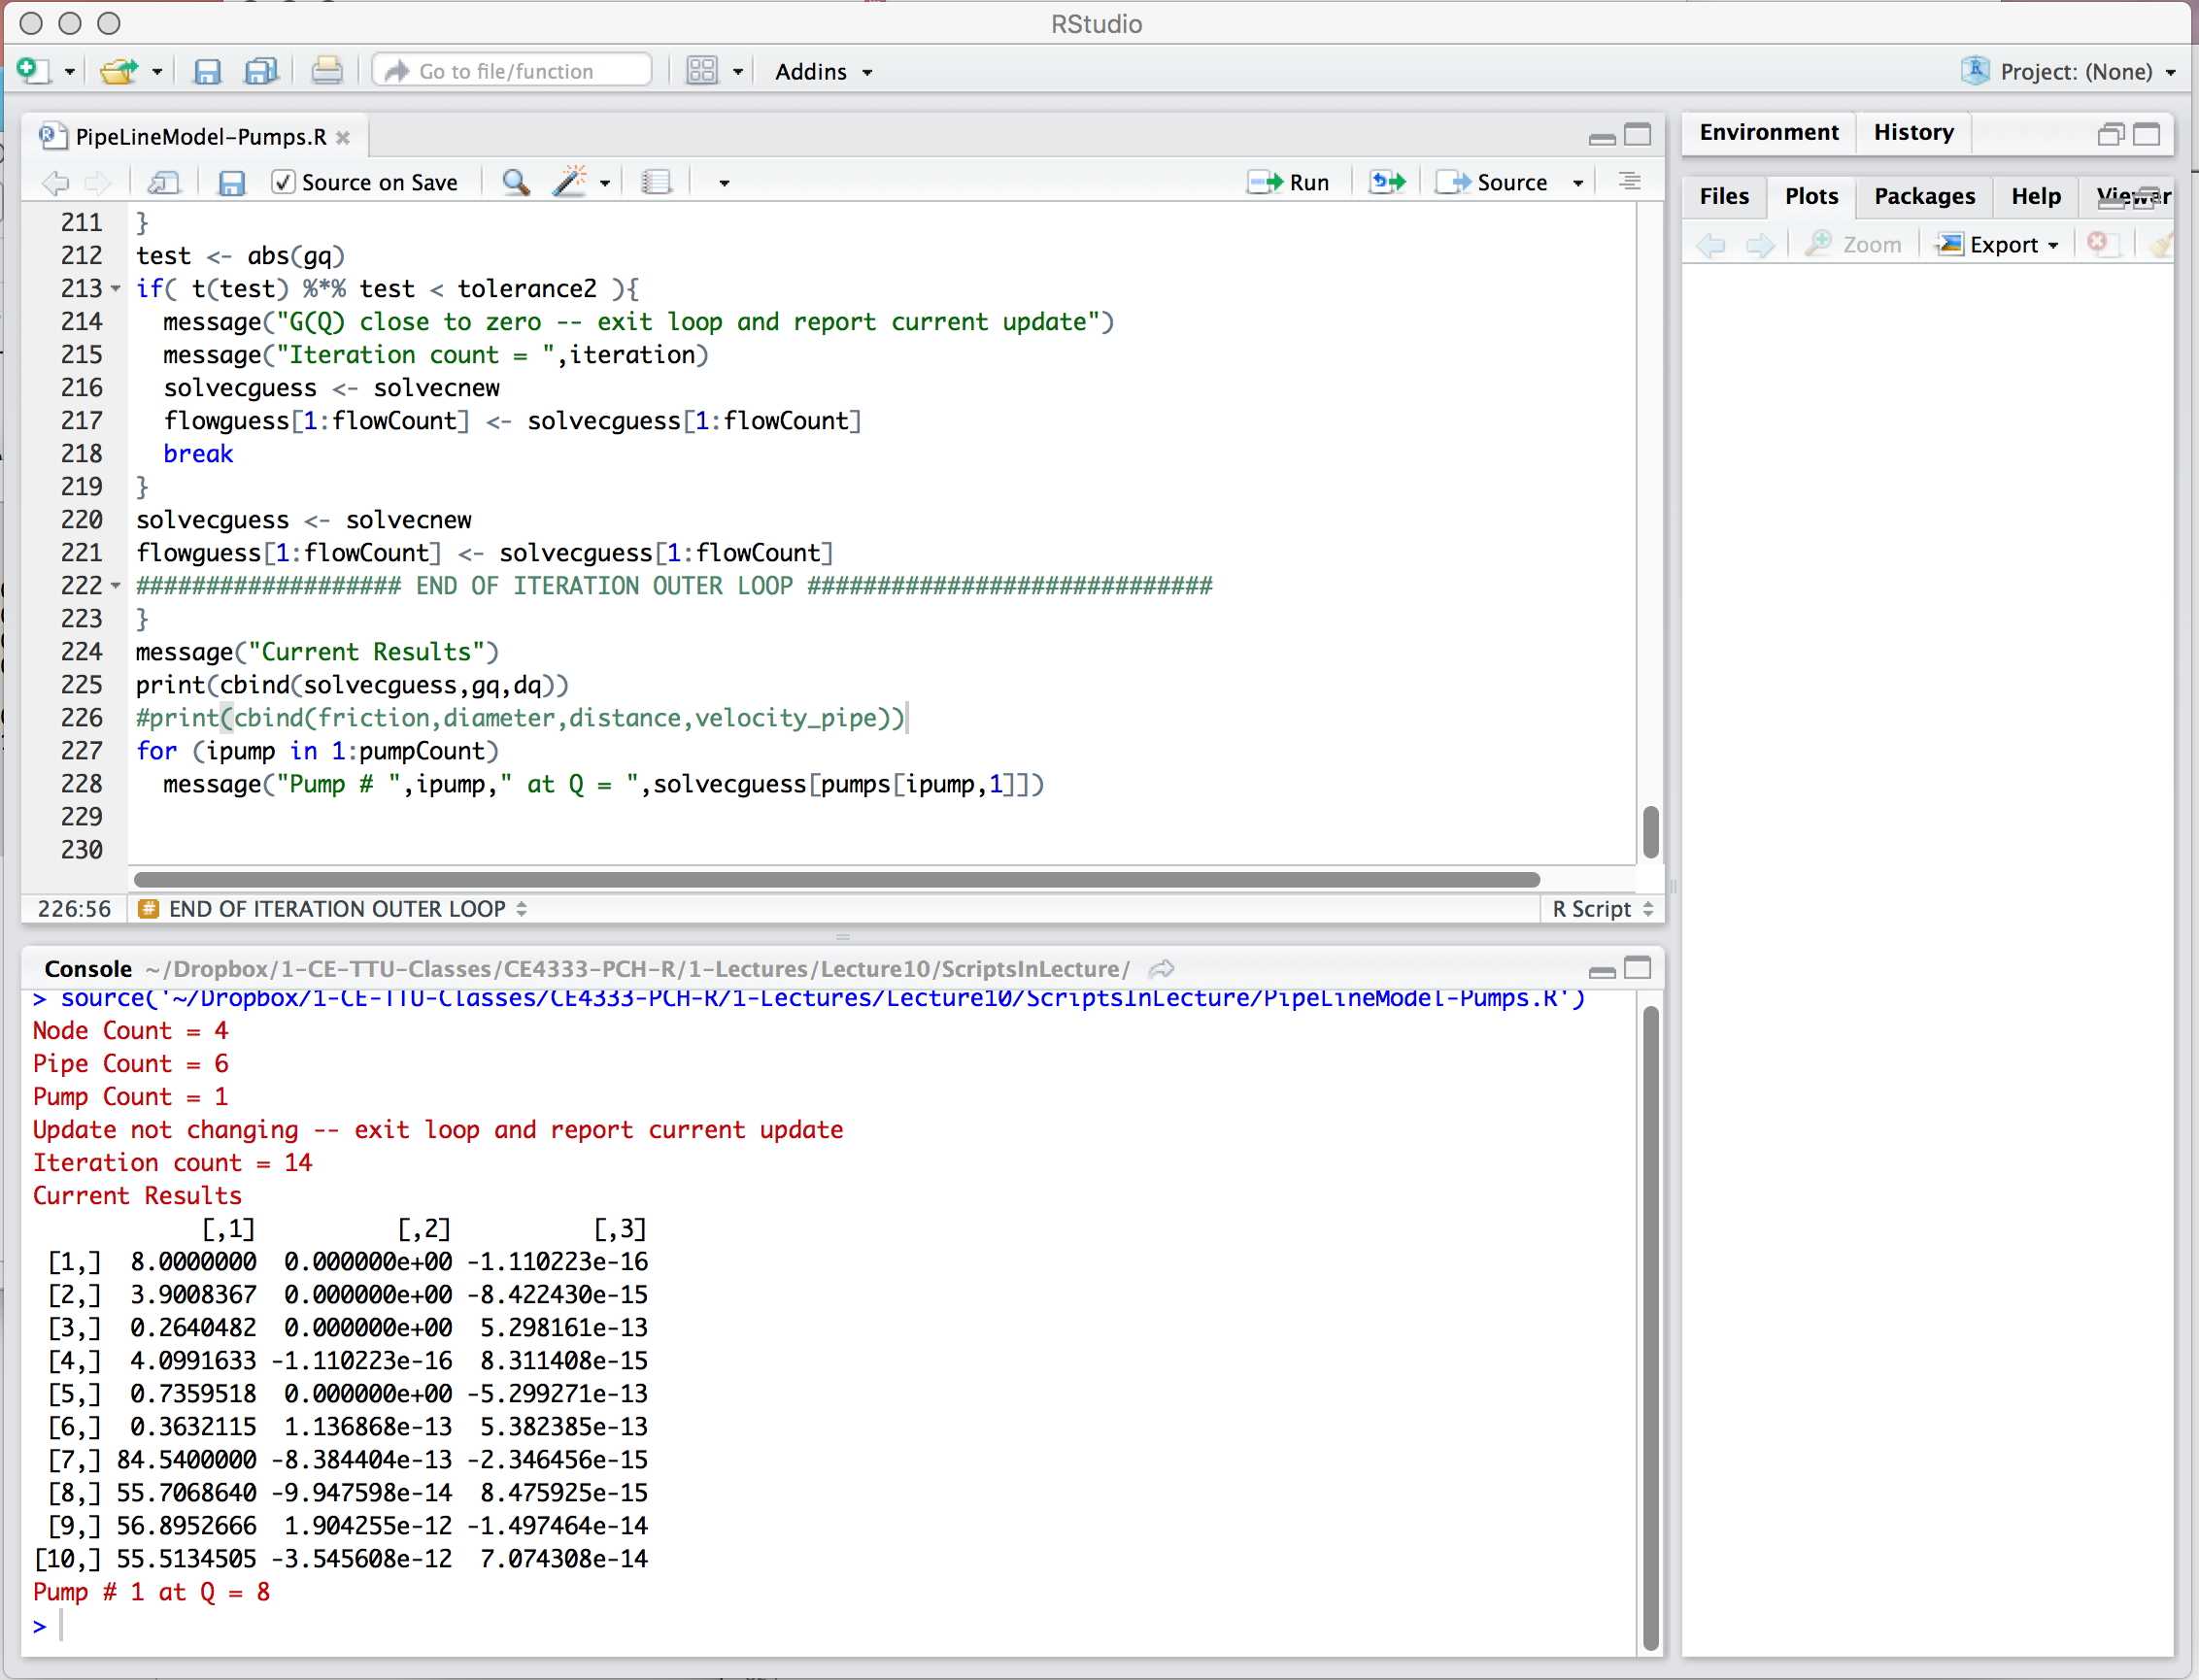
\includegraphics[width=6in]{./10-PumpsAndValves/PipeNetPumpInR.jpg} 
   \caption{Pipe Network with a Pump}
   \label{fig:PipeNetPumpInR}
\end{figure}

\begin{lstlisting}[caption=Input file with pumps at link\#1 in a pipeline network \\ , label=lst:InputWithPump]
1  <== how many pumps
4
6
1.00 0.67 0.67 0.67 0.67 0.5  <== link #1 needs values as placeholders, but are not used
800 800 700 700 800 600
0.00001 0.00001 0.00001 0.00001 0.00001 0.00001
0.000011
1 1 1 1 1 1
1 -1 0 -1 0 0
0 1 -1 0 0 1
0 0 0 1 -1 -1
0 0 1 0 1 0
0 4 3 1 0 0 0 0 0 0
1 100.54 0.25 2.0  <== Pump Link ID, H\_shutoff, K\_pump, Exponent
\end{lstlisting}   

Figure \ref{fig:PipeNetPumpInR} is a screen capture of the example problem run in \textbf{R Studio}.  
The script produces the correct flow values, and the pump specified was intended to match the previous problem closely in that it produces enough head so that node N1 has nearly the same head value as the problem without a pump.

\subsubsection{Fitting (Minor) Losses}
In addition to head loss in the conduit, other losses are created by inlets, outlets, transitions, and other connections in the system.   In fact such losses can be used to measure discharge (think of the orifice plate in the fluids laboratory).  The fittings create additional turbulence that generates heat and produces the head loss.

Equation \ref{eqn:minor-loss-model} is the typical loss model
\begin{equation}
h_{minor} = K \frac{V^2}{2g}
\label{eqn:minor-loss-model}
\end{equation}
where $K$ is called a minor loss coefficient, and is tabulated (e.g. Table \ref{tab:minor-loss-coefficients}) for various kinds of fittings.

\begin{table}[ht!]
   \centering
   \caption{Minor Loss Coefficients for Different Fittings}
   \footnotesize
\begin{tabular}{p{3in}p{.6in}}
Fitting Type & $K$ \\
\hline
\hline
Tee, Flanged, Line Flow&0.2\\
Tee, Threaded, Line Flow&0.9\\
Tee, Flanged, Branched Flow&1.0\\
Tee, Threaded , Branch Flow&2.0\\
Union, Threaded&0.08\\
Elbow, Flanged Regular $90^o$&0.3\\
Elbow, Threaded Regular $90^o$ &1.5\\
Elbow, Threaded Regular $45^o$ &0.4\\
Elbow, Flanged Long Radius $90^o$ &0.2\\
Elbow, Threaded Long Radius $90^o$ &0.7\\
Elbow, Flanged Long Radius $45^o$ &0.2\\
Return Bend, Flanged $180^o$ &0.2\\
Return Bend, Threaded $180^o$ &1.5\\
Globe Valve, Fully Open&10\\
Angle Valve, Fully Open&2\\
Gate Valve, Fully Open&0.15\\
Gate Valve, 1/4 Closed&0.26\\
Gate Valve, 1/2 Closed&2.1\\
Gate Valve, 3/4 Closed&17\\
Swing Check Valve, Forward Flow&2\\
Ball Valve, Fully Open&0.05\\
Ball Valve, 1/3 Closed&5.5\\
Ball Valve, 2/3 Closed&200\\
Diaphragm Valve, Open&2.3\\
Diaphragm Valve, Half Open&4.3\\
Diaphragm Valve, 1/4 Open&21\\
Water meter&7\\
\hline
\end{tabular}
\normalsize
\label{tab:minor-loss-coefficients}
\end{table}

The use is straightforward, and multiple fittings are summed in the loss term in the energy equation.
In practical computation, these losses make the most sense when associated with a particular pipe.  
If we rewrite the loss equation
\begin{equation}
h_{minor} = \frac{K}{2g} \frac{16Q^2}{\pi^2 D^4}
\label{eqn:minor-loss-model-discharge}
\end{equation}
we see that these terms can be added to a pipe either as an additional loss term and placed in the augmented matrix in the same way as the other loss term.

\subsubsection{Extracted Head --- Turbines}
The head recovered by a turbine is also an ``added head'' but appears on the loss side of the equation.   Equation \ref{eqn:turbine-power} is the power that can be recovered by a turbine (again using the concept of ``water-to-wire'' efficiency is 
\begin{equation}
P=\eta Q\rho g h_t
\label{eqn:turbine-power}
\end{equation}
An approach similar to pumps would be employed --- the effort in all these cases is to represent the hydraulic components as a loss factor so the non-linear solver we have already built can be used.  

%\subsection{Exercises}
%\begin{enumerate}
%\item Build a script that includes a pump that supplies the network at the upper left corner and determine the flow distribution in Figures \ref{fig:pipe-net} and \ref{fig:pipe-net-loops}.  
%
%\begin{figure}[h!] %  figure placement: here, top, bottom, or page
%   \centering
%   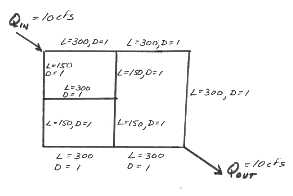
\includegraphics[width=4.5in]{./10-PumpsAndValves/pipe-net.jpg} 
%   \caption{Pipe network for illustrative example with supply and demands identified.  Pipe lengths (in feet) and diameters (in feet) are also depicted.}
%   \label{fig:pipe-net}
%\end{figure}
%
%\begin{figure}[h!] %  figure placement: here, top, bottom, or page
%   \centering
%   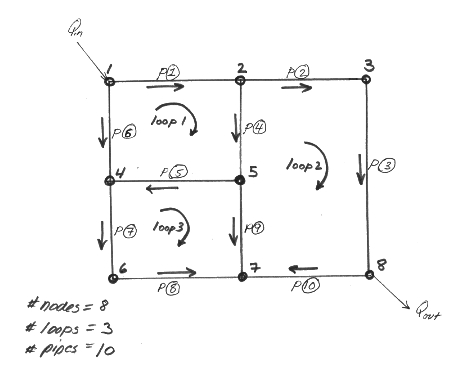
\includegraphics[width=4.5in]{./10-PumpsAndValves/pipe-net-loops.jpg} 
%   \caption{Pipe network for illustrative example with pipes and nodes labeled.}
%   \label{fig:pipe-net-loops}
%\end{figure}
%
%Assume the supply to node N1 is a pump with the following characteristic curve
%\begin{equation}
%h_p = 318.11 - 0.25\times Q^{1.86}
%\end{equation}
%The pump supplies from a reservoir with total head of $0.0$ feet.
%
%In your solution you are to supply
%\begin{enumerate}
%\item An analysis showing the development of the node-arc incidence matrix based on the flow directions in Figure \ref{fig:pipe-net-loops},
%\item The input file you constructed to provide the simulation values to your script,
%\item A screen capture (or output file) showing the results,
%\item The pumping rate of the pump, and
%\item The total heads at each node.
%\end{enumerate}
%
%\end{enumerate}
